%TC: macro \marginfootnote [other]
%TC: envir SCfigure [] other
%TC: macrocount beginSCfigure [figure]
\documentclass[11pt,twoside]{report}
\usepackage{preamble}
\setcounter{chapter}{0}
\graphicspath{{../img/}}
\def\includebibliography{}

\externaldocument{background}
\externaldocument{supercooled-liquids}
\externaldocument{morphometric-framework}
\externaldocument{morphometric-applications}
\externaldocument{resummation}
\externaldocument{aerosols}

\begin{document}
\chapter{Introduction}
%\epigraph{Everything starts somewhere, though many physicists disagree.}{Terry Pratchett, \emph{Hogfather}, (1996).}
\epigraph{I'm being quoted to introduce something, but I have no idea what it is and certainly don't endorse it.}{Randall Munroe, \emph{XKCD}, (2018).}

\begin{SCfigure}
  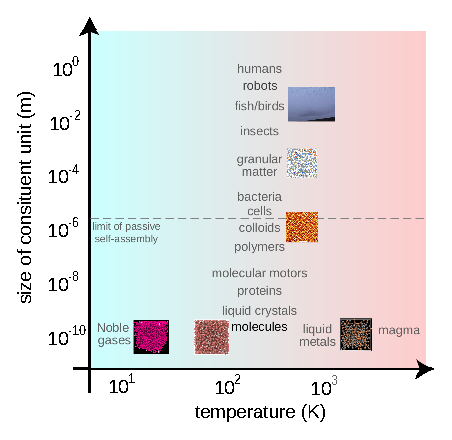
\includegraphics[width=0.75\linewidth,outer]{soft-matter}
  \caption[A loose hierarchy of systems in soft matter]{
    The various systems studied in soft matter, featuring an impressive range of length and temperature scales.
    Every system possesses features in common with liquids, if not actually a liquid themselves.
    Small systems can be dynamically driven through entirely passive sources, with temperature being the prototypical example in thermal systems.
    By contrast, larger systems require active sources of fluctuations to self-assemble, from e.g.\ external driving forces in granular matter or chemical reserves in living systems.
    Image courtesy of Ref.\ \cite{RoyallSoftMatter}.}
  \label{fig:soft-matter}
\end{SCfigure}

It is a matter of some debate over what is precisely meant by ``soft matter'', and how to demarcate the various systems studied.
%I normally introduce this field by taking a deep breath, and then listing the vast range of ...
In introducing this field one normally takes a deep breath, then lists the vast range of topics studied, before drawing inferences over what their quintessential features are; this is an inherently subjective procedure so the boundaries of the field are necessarily fuzzy.
In this vein, soft matter encompasses foams, gels, dispersions, liquid crystals, polymer solutions, polymer melts, granular materials, complex plasmas, active matter and many more systems of fundamental, practical and aesthetic importance.
%% \begin{itemize}
%% \item Foams,
%% \item Gels,
%% \item Dispersions,
%% \item Liquid crystals,
%% \item Polymer solutions and melts,
%% \item Granular materials,
%% \item Complex plasmas,
%% \item Biological and active matter, and
%% \item Many more systems of fundamental, practical and aesthetic importance.
%% \end{itemize}
A widely proposed definition to unify these disparate topics postulates that a soft matter system possesses energy scales accessible to fluctuations  \cite{LubenskySSC1997}, whether this involves spontaneous thermal fluctuations in passive systems or those due to driving forces in active systems.
In each example, the interactions involved are weak enough relative to the source of fluctuations that flow is possible, though the physical processes and chemistry involved can become arbitrarily complex allowing for incredible diversity of phenomena.
In some sense, this idea is best captured with \emph{vaguer} statements, driving a prominent worker in the field to describe soft matter as ``liquids with bits in them'' \cite{Poon2018}.

As a rule of thumb, increasing the size of the constituent components in soft matter systems results in more complex interactions and a greater diversity of phenomena; the various systems are arranged in a loose hierarchy of complexity in Fig.\ \ref{fig:soft-matter}, with molecular systems at the bottom and living things at the top.
In the context of this hierarchy,
%Confusingly, the simplest liquids%
%are often not considered a part of soft matter even though temperature is their defining energy scale.
%So in some sense, soft matter can be more easily understood with \emph{vaguer} statements; a prominent worker in the field describes soft matter as ``liquids with bits in them'' \cite{Poon2018}.
%\todo{Place in Paddy's figure. Redefine soft matter with liquids included.}
the deepest and most universal questions then reside at the level of the simplest liquid%
\marginfootnote{By which we mean those formed by the noble gases at high densities.}.
%, regardless of whether one considers it as a subset of soft matter or as its historical antecedent.
Unsurprisingly, liquids have been thoroughly explored in their long history of study, though fundamental open questions remain concerning their dynamical behaviour at high densities.
To initiate this discussion we will introduce \emph{the} archetypal model for simple liquids: hard spheres.

The hard sphere interaction energy is simply defined by forbidding any configurations where spheres mutually overlap%
\marginfootnote{I like to imagine them as ideal billiard balls, without any dissipative forces so they continue to bounce off one another forever.},
that is
\begin{equation}\label{eq:hs-interaction}
  u(r) =
  \begin{cases}
    \infty & \; r < \sigma \\
    0 & \; \textrm{otherwise},
  \end{cases}
\end{equation}
where $\sigma$ is the diameter of the each sphere.
No chemical bonds are possible in the absence of any attractions so this represents a kind of \emph{zeroth-order} approximation to real fluids; nonetheless, atoms and molecules do feature sharp short-ranged repulsions so this is a reasonable starting point.
Furthermore, this oversimplified model has historically, and counterintuitively, represented the frontiers in our understanding of real liquids.
To illustrate this we consider the van der Waals equation of state for real gases.
This \emph{mean-field theory} characterises a system of $N$ particles contained in a volume $V$ as
\begin{equation}\label{eq:van-der-waals}
  \frac{p - a N}{k_B T} = \frac{N}{V - b N}
\end{equation}
where $p$ is the pressure, $k_B$ is the boltzmann constant, $T$ as temperature, and with $a,b$ as perturbations from the ideal gas law due to the interactions.
We have written this equation such that the left-hand side contains \emph{liquid-like} modifications to the pressure due to the attractions, whereas the right-hand side contains \emph{gas-like} perturbations from the reduction in the accessible volume due to short-range repulsions.
It was widely believed that improvements to this theory would require sophisticated treatments of the \emph{attractions}, however history has shown that it was the treatment of the \emph{repulsions} which were lacking \cite{WidomS1967,Hansen2013,Santos2016}.
Simple liquids can to a large extent be considered as weak perturbations to the hard sphere model; as such, the left-hand side of \eqref{eq:van-der-waals} is reasonably accurate, but the right-hand side must be refined to account for the non-trivial effects of exclusion \cite{Hansen2013}.

%They thus serve as a foundational toy model for fluids in a similar way the Ising model is \emph{the} system for ferromagnetism and critical phenomena.

\begin{SCfigure}
  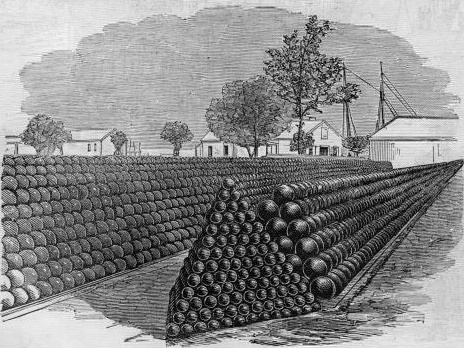
\includegraphics[width=0.75\linewidth,outer]{cannonballs}
  \caption[Close packed cannonballs]{
    Sketch of cannonball piles at Fortress Monroe.
    The stacking structure is an example of close packing, the densest arrangement of hard spheres in three dimensions.
    The ball positions are consistent with sites of a face-centred cubic lattice, similar to that seen in crystal structures.
    Image by Stacy, \emph{Harper's weekly} (1861)}
  \label{fig:fcc}
\end{SCfigure}

As the foundational model for liquids, hard spheres serve as a good touchstone for progress (and controversies) within liquid state physics and, by extension, soft matter.
We will focus our discussion of established properties on the hard sphere phase diagram.
As the hard sphere potential \eqref{eq:hs-interaction} is everywhere zero or divergent, temperature has no effect%
\marginfootnote{The velocities will be trivially rescaled by temperature, but this will not affect the static structure.}
on the thermodynamics and we say the system is \emph{athermal}.
The phase diagram is thus reduced to a single control parameter: the (number) density $\rho = N/V$.
For convenience, and to emphasise the geometric nature of hard spheres, it is usual to work with a normalised density: the \emph{volume fraction}, the volume of space occupied by the spheres i.e.\
\begin{equation}\label{eq:hs-volume-fraction}
  \eta
  =
  \rho \omega_d \left( \frac{\sigma}{2}\right)^d,
\end{equation}
where $\omega_d$ is the volume of a $d$-dimensional ball of unit radius e.g.\ $\omega_3 = 4\pi / 3$.
From its definition we know the volume fraction must be bounded from above by $\eta < 1$ where all space would be perfectly tiled, although in practice tighter upper bounds can be placed from the constraints of spherical packings.
The largest density achievable without causing spheres to overlap is called the \emph{close packing} limit, and in $d = 3$ corresponds to the face centred cubic (FCC) lattice (Fig.\ \ref{fig:fcc}), occurring at $\eta_\mathrm{CP} = \pi / (3\sqrt{2}) \sim 0.74$.
This happens to coincide with a crystal structure observed in real systems, so by analogy we might postulate the existence of a thermodynamic phase transition separating this ordered state from the disordered state around the dilute limit $\eta \to 0$ where ideal gas behaviour is recovered.

\begin{SCfigure}
  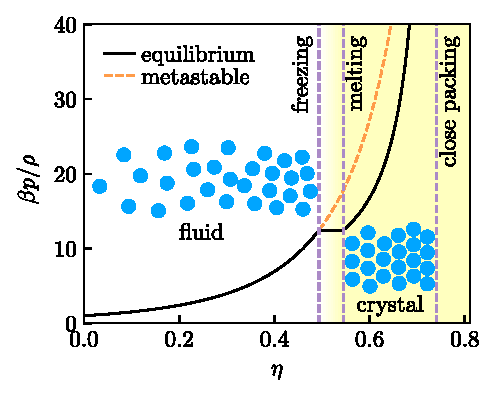
\includegraphics[width=0.85\linewidth,outer]{hs-phase-diagram}
  \caption[The hard sphere equation of state and phase diagram]{
    The hard sphere equation of state in $d=3$ in terms of volume fraction, including the metastable branch.
    The one-dimensional phase diagram is overlaid, with the volume fractions of freezing and melting taken as $\eta_f \sim 0.494$ and $\eta_m \sim 0.545$ respectively \cite{HooverJCP1968}.
    Close packing occurs at $\eta_\mathrm{CP} \sim 0.74$.
    The equations of state were adapted from Refs.\ \cite{CarnahanJCP1969,SpeedyJPCM1998,BannermanJCP2010}.
  }
  \label{fig:hs-phase-diagram}
\end{SCfigure}

Written in terms of volume fraction, the van der Waals equation \eqref{eq:van-der-waals} for $d$-dimensional hard spheres adopts the simpler form%
\marginfootnote{The coefficient of $2^{d-1}$ in this form can be obtained by recognising that leading-order corrections to the ideal gas law involves the \emph{excluded volume}, i.e.\ that excluded to the centre of a test particles which modifies the occupied volume by $2^d$ by doubling the radius.
  This has to be divided by two to avoid double counting the particle interactions, giving the final result.}
\begin{equation}\label{eq:van-der-waals-hs}
  \frac{\beta p}{\rho} = \frac{1}{1 - 2^{d-1} \eta}
\end{equation}
where $\beta = (k_B T)^{-1}$, and we recognised that $a = 0$ because hard spheres have no attractions.
This theory features no singularities until $\eta = 2^{1-d}$ where the pressure diverges, so it predicts no thermodynamic phase transitions and contradicts the existence of a close packing limit at $\eta_\mathrm{CP} \sim 0.74$ in $d=3$.
By contrast, the actual phase diagram (Fig.\ \ref{fig:hs-phase-diagram}), determined from simulations \cite{AlderJCP1957,WoodJCP1957,HooverJCP1968} and colloidal experiments \cite{PuseyN1986}, shows that the hard sphere system remains a liquid%
\marginfootnote{Strictly speaking there is no distinction between a liquid and a gas phase in hard spheres because the phase diagram does not have a critical point.
  As such, to be precise we should refer to the isotropic phase as a \emph{fluid}.
  However, we will always be focusing on the high density fluid, which serves as the starting point for descriptions of real liquids, so we can justify using `liquid' and `fluid' interchangeably.}
up to $\eta_f \sim 0.494$ whereupon it undergoes a freezing transition to an ordered phase with an accompanying melting transition at $\eta_m \sim 0.545$ \cite{HooverJCP1968}.
%Controversial, .
This result was not immediately accepted by the community, even though these simulation studies are generally considered definitive in hindsight.

%The hard sphere freezing transition suggests the counterituitive notion that billiard balls will spontaneously order into a crystal at high densities.
In everyday scenarios crystallisation typically occurs as one lowers temperature, and the classroom explanation posits that the crystal is favoured due to \emph{attractions} between molecules.
In the absence of any attractions in hard spheres, we find that \emph{entropy} must drive crystallisation.
Part of the reason people could not believe that the crystal is entropically favoured, is because we often (mistakenly) identify entropy as a measure of disorder making it counterintuitive for an ordered phase to be favoured.
In reality entropy is more subtle: the crystal may be more ordered than the liquid, with a lower \emph{configurational} entropy, however entropy includes other contributions.
At high densities, the penalty paid for being locked into the crystal is offset by a \emph{vibrational} entropy, because each particle has more available space for motion.
%\marginfootnote{This is a free volume argument which accounts for most of the driving force behind crystallisation in hard spherse, although subleading collective effects will also be present.}.
The net entropic effect leads to the crystal being favoured over the liquid at high densities, giving the phase diagram that we know today (Fig.\ \ref{fig:hs-phase-diagram}).

A similar effect is seen in balls floating on water as in e.g.\ peas boiling in a saucepan or shade balls covering a reservoir (Fig.\ \ref{fig:shade-balls}).
The hard interactions between the balls causes%
\marginfootnote{In an attempt to find an everyday example, I have taken liberties with the interaction being purely hard; I suspect that floating balls feature effective attractions because of \emph{hydrodynamic} interactions at the water surface.}
them to `crystallise' at high densities as can been seen in the figure.
Strictly speaking these are not crystals in the sense of long-range \emph{translational} order, instead they are said to possess long-range \emph{orientational} order.
This subtlety emerges because the floating balls are confined to the water surface making them effectively two dimensional.
In thermal systems, fluctuations are strong enough in two dimensions to overcome truly long-ranged positional ordering \cite{MerminPRL1966,MerminPR1968}; as macroscopic objects, the floating balls are not strictly thermal but we can expect reminiscent behaviour emerging from any fluctuation source e.g.\ water waves.

\begin{SCfigure}
  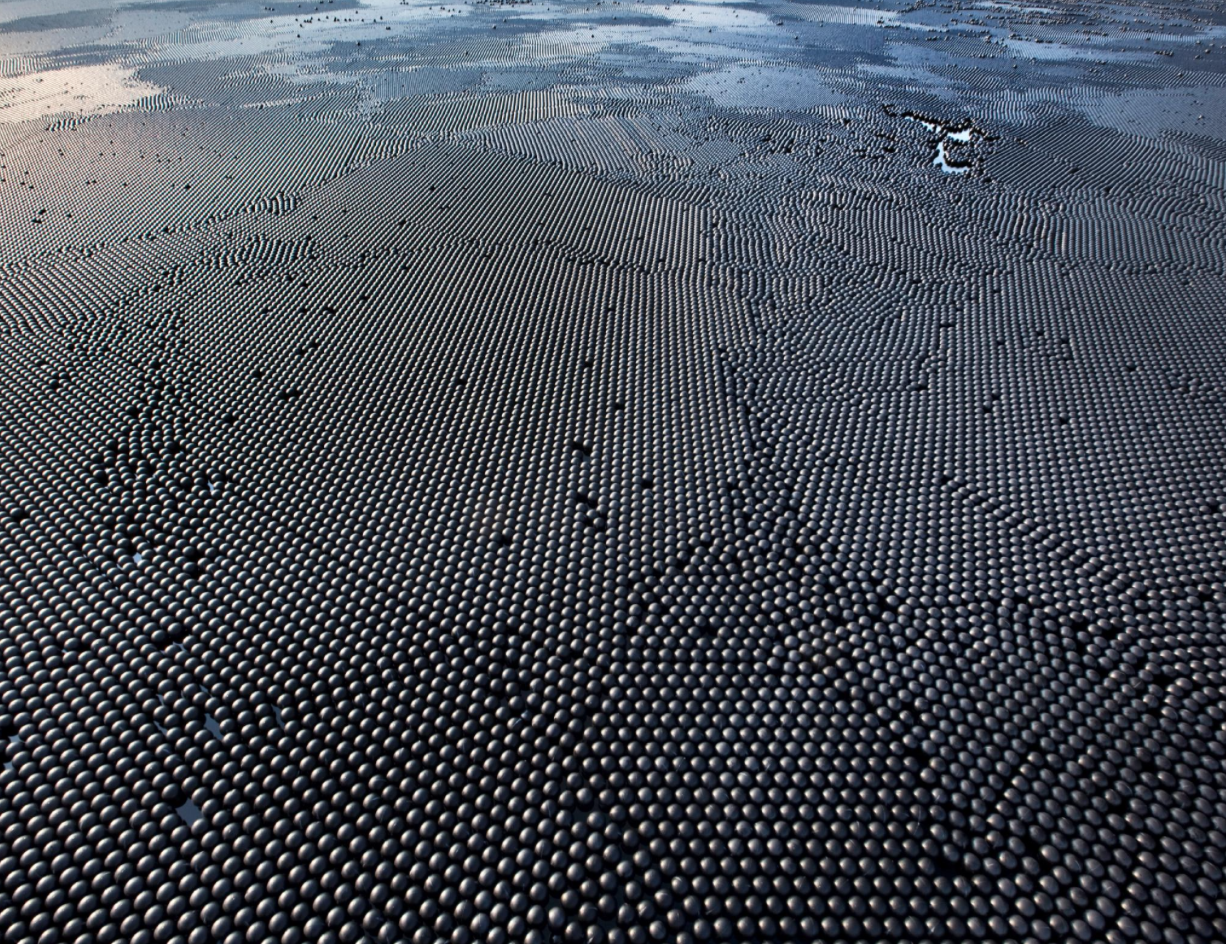
\includegraphics[width=0.75\linewidth,outer]{shade-balls}
  \caption[Shade balls floating on water: a 2d `crystal']{
    Shade balls covering the Los Angeles reservoir to cool the water, preventing evaporation, and inhibit harmful light-activated chemical reactions at the water surface.
    As macroscopic objects these balls interact as hard spheres, and they spontaneously form long-ranged orientational order seen as hexagonal domains.
    This is reminiscent of crystallisation in atomic systems.
    Image by Gerd Ludwig, \emph{National Geographic} (2007).}
  \label{fig:shade-balls}
\end{SCfigure}

%% We have extolled the virtues of hard spheres, however this should not be interpretted as saying that this model system capture \emph{all} of the physics of real systems: it is a toy system after all.
%% As an example of physics they do \emph{not} capture, consider the critical point of real liquids.
%% Liquid-gas critical phenomena emerges from a competition between attractive and repulsive forces, with divergent fluctuations at the critical point.
%% It is thus impossible for a system with purely repulsive interactions, like hard spheres, to feature a critical point.
%% That being said, many theories predict critical phenomena quite well by taking a hard sphere potential and incorporating a mean-field like attractive perturbation \cite{?} so a hard sphere system provides a good reference point.

%% Hard spheres exist in more than just a theorist's imagination: they can be experimentally realised in colloidal experiments.
%% Colloidal suspensions are mixtures of solute immersed in a solvent composed of much smaller particles.
%% Colloidal particles are typically at the micron-scale.
%% These typically feature complex interactions \cite{Royall?,?,?} however these can be tailored to closely approximate hard sphere like interactions through steric stabilisation.
%% \todo{What is an aerosol? What is a dispersion?}
%% Colloidal experiments closely match hard simulations and theoretical predicitons \cite{?}.
%% Notably one can determine the phase diagram see Fig.\ \ref{fig:hs-phase-diagram}.
%% Note the glass at very high densities.

Now that we have given an overview of the firmly established bulk phase behaviour of hard spheres, we can turn to address the questions which remain unresolved.
So far we have only discussed the \emph{equilibrium} properties of hard spheres which are well-described by theory.
In equilibrium, a great deal is even known about the \emph{inhomogeneous} liquid, e.g.\ in confinement \cite{GonzalezJCP1998}, thanks to advances in density functional theory \cite{RosenfeldPRL1989,RothJPCM2010}.
By contrast, there are still much debate surrounding the nature of the \emph{metastable} phase in hard spheres, especially concerning its dynamical properties.
%We now turn to the central questions still unresolved concerning the hard sphere system, which focus on their metastable properties at high densities.
%As the most widely studied model interaction potential we know a lot about its equilibrium structure (phase diagram) in bulk and even inhomogeneous thanks to density functional theory \cite{?,?,?}.
%However, its behaviour off-equilibrium at high densities is hotly debated.
%The two biggest unresolved research topics for this subject:
The metastable phase is the continuation of the liquid phase above the melting point, shown by a dashed line in Fig.\ \ref{fig:hs-phase-diagram}.
We refer to this branch as the \emph{supercooled liquid} in analogy to the metastable phase of real liquids which are formed by cooling below their freezing temperature; in this sense we think of increasing density as equivalent to lowering the temperature.

The supercooled liquid is not strictly a phase in the sense of being the free energy minimum, as it will eventually crystallise, however it has many features in common with equilibrium phases.
In particular, the supercooled liquid is long-lived and it eventually reaches a steady state with well-defined thermodynamic observables.
In simple terms, supercooled liquids are thermodynamically indistinguishable from that of an equilibrium phase \emph{until} they spontaneously crystallise.
However, supercooled liquids profoundly differ from ordinary liquids in their \emph{dynamical} properties, which are the least understood aspects of simple liquids and we discuss more below.
%We will leave detailed discussion of the specific properties of supercooled liquids until chapter \ref{chapter:glass}, as for now we only wish to briefly introduce the key questions posed.
%\todo{Demphasise thermodynamics, emphasise dynamics.}
%so we will find it useful to describe it with similar language.

As we see it, the two central topics regarding the metastable liquid are:
\begin{enumerate}
\item \emph{Fate of the liquid branch}: if crystallisation could (somehow) be circumvented, what is the ultimate fate of the supercooled liquid as one increases the density?
  Related to this is the nature of the out-of-equilibrium state: the \emph{glass}.
\item \emph{Nucleation}: given that the crystal is the ground state above the freezing density, can we describe the kinetic pathway by which the liquid orders into the crystal?
\end{enumerate}
Each question is complicated by a remarkable change in the timescales involved, requiring new ideas to approach them.
Regarding nucleation, the rates predicted by theory and experiments differ by some $\sim$12 orders of magnitude, which is claimed to be the second worst disagreement%
\marginfootnote{With the first being the \emph{vacuum catastrophe}, the difference of $\sim$120 orders of magnitude between predicted vacuum energy density and observations of astronomers \cite{Hobson2006}.
In this context, nucleation predictions become remarkably accurate.}
between theory and experiment in all of physics \cite{RussoSM2013}.

In the supercooled liquid the time to reach the steady state, or `equilibrium', dramatically increases with density until it becomes effectively infinite above a glass transition%
\marginfootnote{This is typically taken to occur around $\eta_g \in [0.58, 0.60]$, although the exact point where the system falls out of equilibrium will depend on many factors including the size of the particles in case of colloidal experiments, the specific dynamical rules of a simulation algorithm, and the patience of the observer.}[1.5cm]
where it forms a glass.
If the hard sphere glass is continually compressed to higher densities the pressure will diverge, which is related to \emph{jamming} in granular materials like sand.
Empirically this occurs at \emph{random close packing} (Fig.\ \ref{fig:rcp}) around $\eta_\mathrm{RCP} \sim 0.64$, but as an out-of-equilibrium state this is highly protocol dependent so this density may not be well-defined \cite{TorquatoRMP2010}.
%This is complicated by the fact that as density increases the dynamical timescales increase by $\gtrsim 14$ orders of magnitude, so no ordinary simulation or experiment can probe `equilibrium' properties.
Our focus will be on the `equilibrium' supercooled liquid, although the nature of the glass and jammed states provide important context for our programme, which we will return to in chapter \ref{chapter:glass}.
The central question of this field asks if the relaxation timescale, or viscosity, truly diverges at finite pressure; an equivalent question asks whether there is a thermodynamic transition to an \emph{ideal glass} phase which drives the dynamical slowdown.

\begin{SCfigure}
  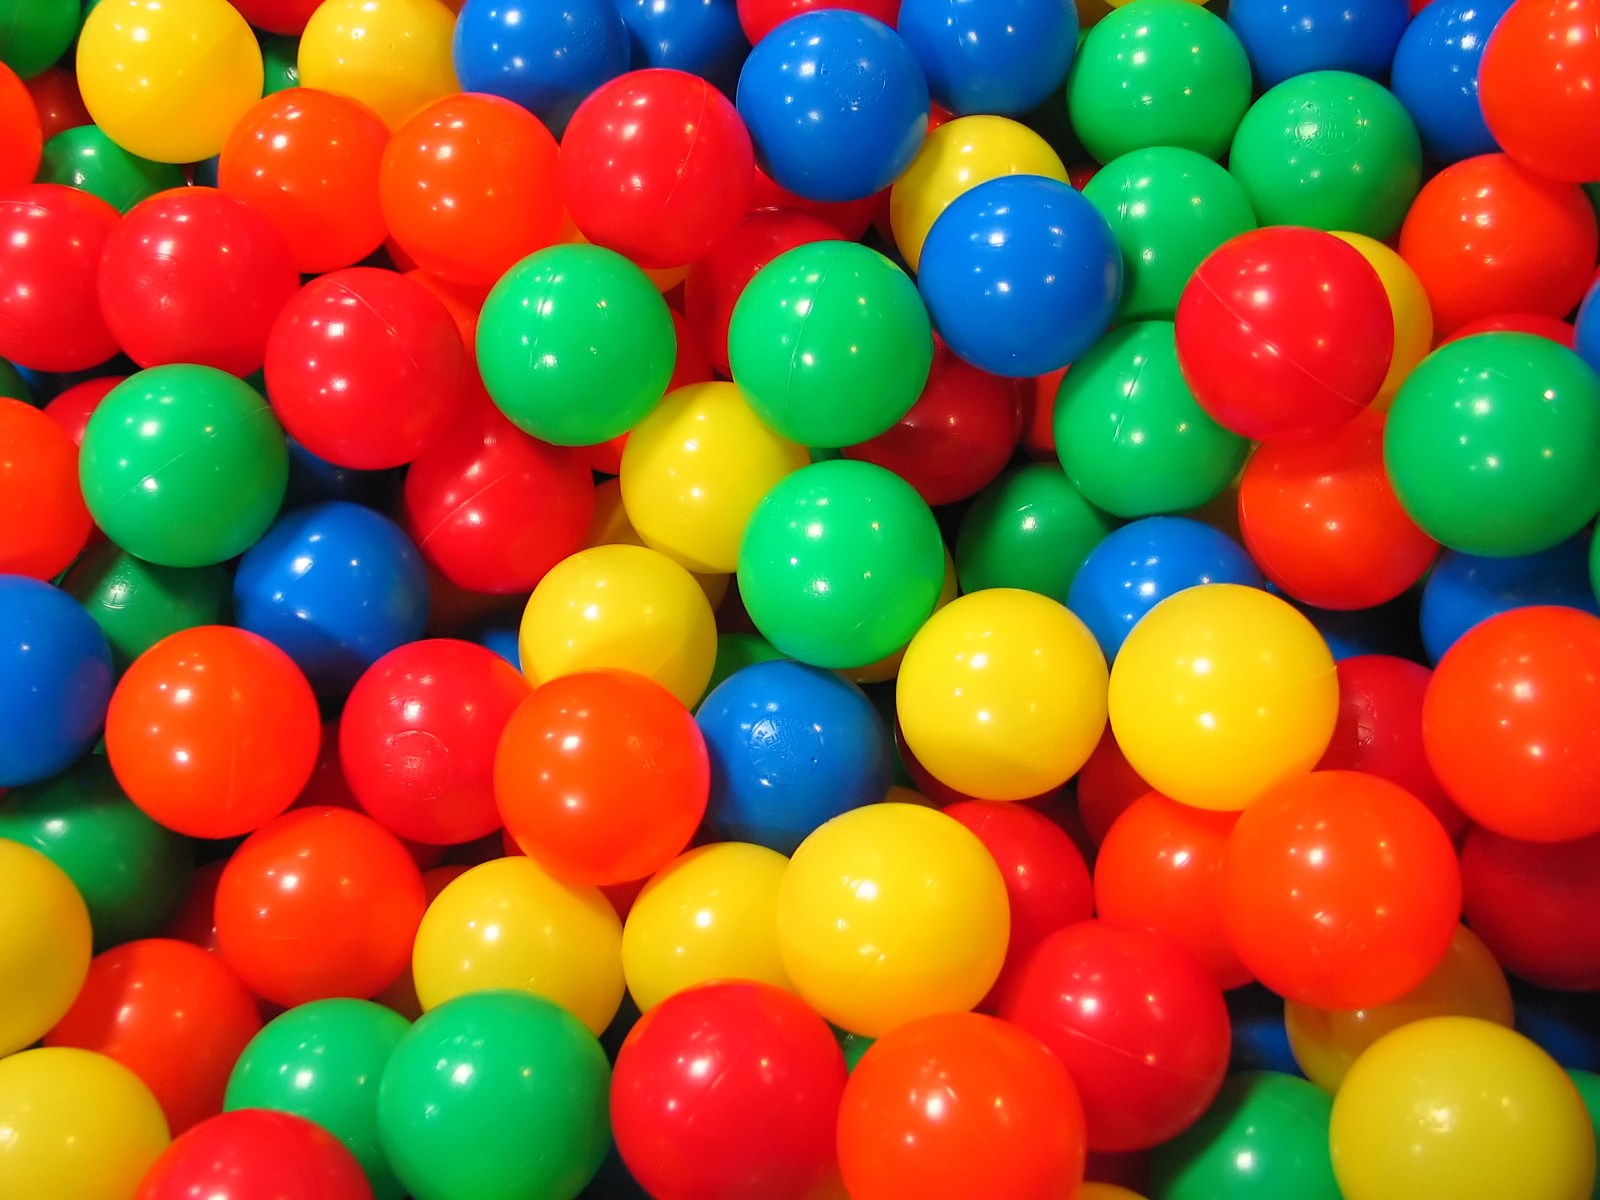
\includegraphics[width=0.75\linewidth,outer]{ball-pit-horizontal}
  \caption[Random close packing in a ball pit]{
    Hard spheres in a ball bit are (approximately) randomly close packed, occurring at a volume fraction $\eta_\mathrm{RCP} \sim 0.64$.
    These disordered packings are minimally rigid until perturbed, by e.g.\ a child jumping in, whereupon many particles are collectively displaced in \emph{avalanches}; disorder in ball pits is thus essential to their function.
    Image by Peter Ong.}
  \label{fig:rcp}
\end{SCfigure}

The goal of this thesis is to advance the methods of treating liquids at high densities, so we aim make a small contribution to addressing both topics above; in chapters \ref{chapter:morphometric-framework}, \ref{chapter:morphometric-applications} and \ref{chapter:resummation} we will develop methods to assess changes in the supercooled hard sphere liquid, while in chapter \ref{chapter:aerosols} we will model nucleation kinetics in drying aerosols.

%% Metastable liquid.
%% Evantually this falls out of equilibrium.
%% In recent years a consensus has been forming.
%% We will return to talk more about glasses and the supercooled liquid this in section \ref{sec:glass} of the literature review.
%For the single-component hard sphere liquid this question is of minimal practical interest, because it is nigh impossible to prevent crytallisation so this is an academic/fundamental question.

In chapter \ref{chapter:background} we will present an overview of liquid state theory, with a special emphasis on correlation functions and geometric methods as these will play a central role in later chapters.
In the following chapter \ref{chapter:glass} we discuss the supercooled liquid in more detail to provide proper context for the first topic outlined above, which is our central motivation.

In chapters \ref{chapter:morphometric-framework} and \ref{chapter:morphometric-applications} we develop our approach to the supercooled liquid: we use the framework of many-body correlation functions to predict the concentrations of local structures in the bulk liquid.
A bulk system with $10^{23}$ particles has too many degrees of freedom to treat effectively, so our approach is to select a subset which remain dynamically relevant.
We will justify this procedure using existing theories of the supercooled liquid discussed in chapter \ref{chapter:background}.
We find that many-body correlations provide the natural framework for this task, and we develop specific theories for treating correlations in the hard sphere liquid in chapter \ref{chapter:morphometric-framework}.
Then in chapter \ref{chapter:morphometric-applications} we develop this into a predictive framework for concentrations of local structural motifs, and dynamical barriers, within the bulk liquid.
Central to these chapters is the \emph{morphometric approach}, an approximation scheme emerging as a synthesis of liquid state theory and geometry, which we will introduce gradually over the course of chapters \ref{chapter:background} and \ref{chapter:morphometric-framework}.
As the final stage in this sequence of connected results, we rederive the morphometric approach in chapter \ref{chapter:resummation} from first principles within liquid state theory to further justify the approach and provide insight into how the approximation may be improved.
%It is not yet known how useful this approach will be in addressing the questions posed above, however the idea of extracting information about a macroscopic system from studying 6--13 particles should, at the very least, be entertaining.

The problem that we solve is actually quite general: given an interaction potential, we want to know what kinds of structures will form in the bulk liquid.
To the best of our knowledge, this has never been done for \emph{any} system.
Admittedly, we repeatedly exploit the simplicity of the hard sphere interaction potential to do this, limiting the applicability to real systems, but it is still a non-trivial problem.
Were this to be generalised to more complex systems, we could imagine the methods being used to facilitate design of new chemical synthesis, tailoring the self-assembly of colloidal particles, or for predicting how proteins fold in aqueous solution.
%One can imagine this method being useful in more complex systems such as protein folding in aqueous solution, predictive self-assembly of complex structures, predictive chemical reactions etc.
Although hard spheres will be our focus, we will indicate possible routes to extending the results throughout, and we will explicitly extend the approach to arbitrary mixtures of hard convex particles in chapter \ref{chapter:resummation}.
%% Self-assembly is an active area of soft matter: it is technologically desirable to tailor the final structure by controlling the building blocks.
%% Imagine assembling nanomachines or artificial cells by controlling the chemistry.
%% It is found that varying the size and shape of hard particles can reproduce all the complexity of the periodic table \cite{Glotzer?,Dijkstra?}.
%% Hard spheres are the simplest such system, so a theory which can treat other geometries is desirable.

Second, our problem is intimately connected to sphere packing problems which are important for the study of granular materials and in computer science where they are essential for coding signals for transmission over noisy channels and potentially for encryption%
\marginfootnote{Notably, encryption using spherical lattices is one potential candidate for post-quantum cryptography \cite{Cohn2016}.}.
Determining the densest possible packing of spheres is a notoriously difficult problems in general \cite{Cohn2016,Conway1999}; the close packing of three-dimensional spheres already discussed was conjectured by Johannes Kepler in 1611, but it took nearly 400 years and a \emph{tour de force} of combined mathematical and computational arguments to actually prove it \cite{HalesAM2005}.
Related questions concern determining the number and nature of rigid packings \cite{Conway1999,Holmes-CerfonSR2016,Holmes-CerfonARCMP2017}, the results of which we use extensively.
Our approach thus provides a connection between sphere packing problems and properties of liquids.

%% We mention some other open problems of hard spheres, that will not be directly addressed though many of the ideas and methods developed in this thesis could transfer.
%% There is a deep connection between hard spheres and computer science.
%% We already mentioned close packing, though this is a hard problem in general.
%% Packing problems have been studied \cite{Cohn2016,Conway1999} and they are notoriously difficult; Kepler conjectured the optimal packing in 3d was the face-centred cubic/hexagonal close packing but it took 300(?check) years to solve this.
%% The final proof was computer aided, and not simple.
%% Packing problems are connected with encoding/encryption.
%% Transmitting a signal requires a way to encode a message across a band(?): if packed too tightly on the band(?) then noise will destroy the signal to it is desirable to optimise the sites for bits \cite{Cohn,?,?}.
%% Additionally, lattice based encryption techniques are one of the alternatives to prime factorisation: the coming development of quantum computers \cite{?,?} would render prime factorisation easy because of Shor's algorithm \cite{Shor?} rendering standard encryption techniques insecure.
%% The techniques developed for the mean-field hard sphere problem have been applied to the perceptron model \cite{?}, and deep-learning neural networks which are naturally high dimensional problems lending themselves to a mean-field treatment \cite{?}.

%% As a secondary goal, The liquids and glass community do not have a great deal of overlap.
%% The glass community , in spite of recent advances in liquids
%% However a small community of .
%% The aim of chapters will be to introduce these ideas into glassy physics.
%% In reflection of this, the literature review of \ref{chapter:background} will focus on methods of liquid state theory.
%% We will be advancing liquids into glasses, so while it is important that we review the paradigms of glassy physics, we will not be using methods developed intrinsically for glasses.

Finally, in chapter \ref{chapter:aerosols} we will change subject to address the nucleation kinetics in drying aerosols.
This project emerged from an opportunity to collaborate with the Bristol Aerosol Research Centre, so it was driven by experimental conditions which are not adequately captured by a purely hard sphere model.
The nucleation theory we employ is identical to that used to describe hard sphere crystallisation, so the questions posed in this applied context are fundamental.
We intended to keep this chapter self-contained, so we save full discussion of nucleation until chapter \ref{chapter:aerosols}.

\ifdefined\includebibliography
  \newgeometry{margin=1in}
  \printbibliography
\fi
  
\end{document}
